%*******************************************************************************
%*******************************************************************************
\chapter{Songbook-Client}
\setcounter{chapter}{2}
\label{chap:songbook-client}
\minitoc
\newpage
%*******************************************************************************
%*******************************************************************************

Le Songbook-Client est interface graphique facilitant la création de
recueils de chansons
personnalisés\footnote{\url{http://www.ohloh.net/p/songbook-client},
  \url{http://github.com/crep4ever/songbook-client}}.

Il est nécessaire d'avoir installé au préalable les dépendances du
songbook lui-même (\refsec{sb:install}). 

Les téléchargements suivant les différents systèmes d'exploitation
sont proposés sur \url{http://www.patacrep.com/static1/downloads}.


%*******************************************************************************
\section{Interface}
%*******************************************************************************

%-------------------------------------------------------------------------------
\subsection{Éléments principaux}
%-------------------------------------------------------------------------------

\begin{figure}
  \centering
  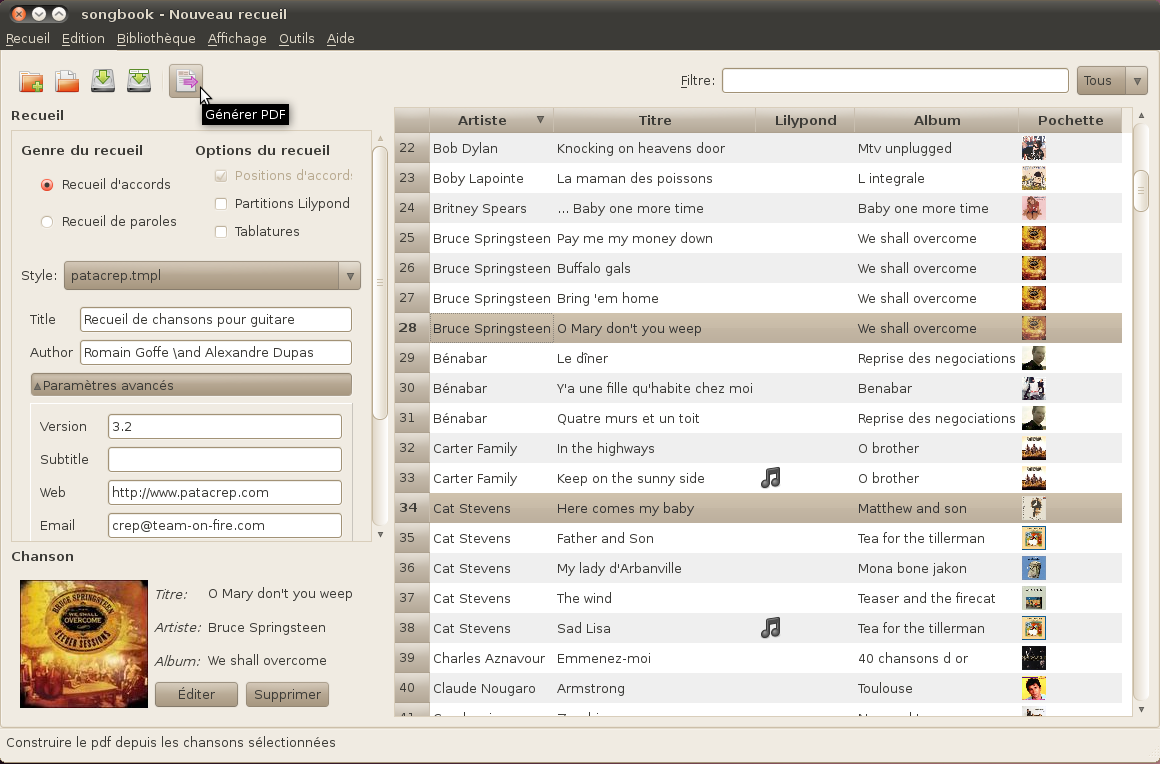
\includegraphics[width=\textwidth]{sbc-v0-3-01}
  \caption{Patacrep Songbook Client~: interface pour la génération de
    recueils de chansons.}
  \label{fig:sb-client}
\end{figure}


%-------------------------------------------------------------------------------
\subsection{La bibliothèque des chansons}
%-------------------------------------------------------------------------------


%-------------------------------------------------------------------------------
\subsection{L'éditeur de chansons}
%-------------------------------------------------------------------------------


%*******************************************************************************
\section{Générer un recueil}
%*******************************************************************************

\paragraph{Sélection des chansons}
Cliquez sur les chansons que vous souhaitez voir apparaitre dans votre
recueil.  Les chansons sélectionnées sont en surbrillance. Utilisez
l'action \Key{Générer PDF} pour générer le pdf disponble depuis le
menu Recueil/Générer ou depuis le bouton à droite dans la barre
d'outils.

\paragraph{Enregistrez votre recueil}
Un recueil est un fichier .sb dans lequel sera enregistré la liste des
chansons sélectionnées ainsi que les options et les champs
personnalisés du recueil lui-même.



%*******************************************************************************
\section{Ajouter une chanson}
%*******************************************************************************

\todo

%*******************************************************************************
\section{Compilation depuis les sources}
%*******************************************************************************

%-------------------------------------------------------------------------------
\subsection{\linux}
%-------------------------------------------------------------------------------

\paragraph{Compilation depuis les sources}

\begin{unix}
  sudo apt-get install build-essential cmake libarchive-dev
  sudo apt-get install qt4-qmake qt4-dev-tools libqt4-sql-sqlite
\end{unix}

\begin{unix}
  git clone git://github.com/crep4ever/songbook-client.git
  cd songbook-client
  make && sudo make install
\end{unix}

%-------------------------------------------------------------------------------
\subsection{\windows}
%-------------------------------------------------------------------------------


%*******************************************************************************
\section{FAQ}
%*******************************************************************************

\paragraph{Comment signaler un bug ?}
Directement sur Github
(\url{http://github.com/crep4ever/songbook-client/issues}) ou via le
forum (\url{http://www.patacrep.com/forum/}).

\paragraph{Erreur Sqlite au démarrage} 
Si vous voyez une boîte de dialogue d'avertissement se lancer au
démarrage de l'application indiquant que le support de sqlite est
nécessaire, vous ne pourrez pas utiliser l'interface. Vérifiez que
votre système dispose bien du support Qt de sqlite (sous
Debian/Ubuntu, il s'agit du paquet \command{libqt4-sql-sqlite}).

\paragraph{Les partitions de solfège n'apparaissent pas}
Si la compilation de votre recueil de chansons n'intègre pas les
partitions malgré l'option \emph{Lilypond} correctement cochée dans les
préférences, vérifiez que Lilypond est bien installé sur votre système. 

\paragraph{La bibliothèque des chansons est vide} 
Vérifiez que le chemin d'accès au patacrep songbook est correctement
renseigné dans Édition/Préférences.  Le chemin indiqué doit contenir
impérativement le makefile et le répertoire \directory{songs/}.

\paragraph{Erreurs après renommage/suppression d'une chanson} 
Un ``make clean'' ou, depuis l'interface, Recueil/Nettoyer devrait
régler le problème. S'il persiste encore, une solution radicale
consiste à supprimer manuellement tous les fichiers \ext{.d} présents
dans \directory{$\sim$/songbook}.

